\section{Impossible Differential Trail on Saturnin}
\begin{frame}{Two impossible Differential Trails}
    \begin{center}
        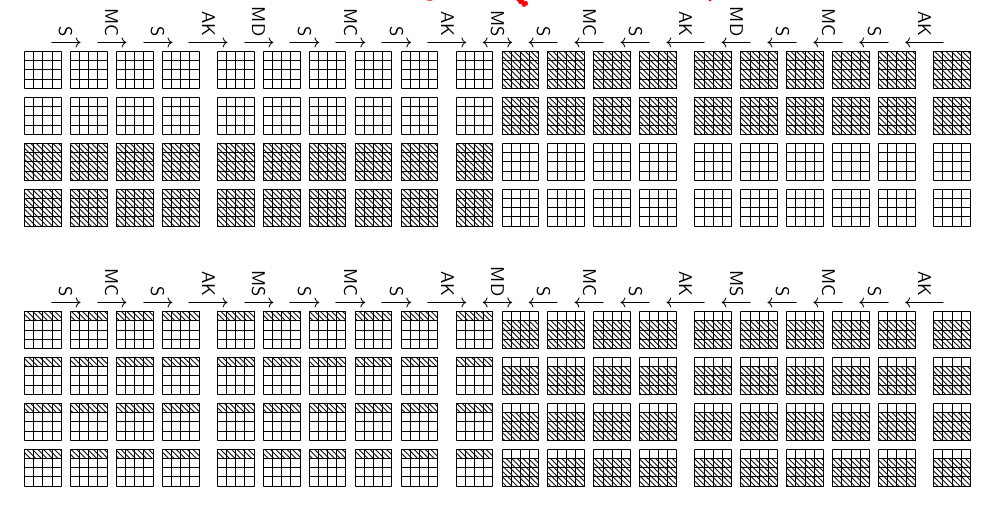
\includegraphics[width=0.85\textwidth,height=0.9\textheight,keepaspectratio]{Images/Figures/imp_diff.png}
    \end{center}
\end{frame}

\begin{frame}{Differential Trail 1}
    \begin{itemize}
        \item Its a 4 round Impossible Differential, meeting in the middle.
        \item Starts with a small number of active nibbles in the state.
        \item We start from the left from the top and the MD step which has SR slice diffuses the sboxes only in the slice
        \item Hence when we start from the bottom, the trail doesnt match with each other.
        \item So the first round starts from even then $x\%4 = 1$ so 4 5 6 7, becuase we are using SR slice.
        \end{itemize}
    \end{frame}
    
    \begin{frame}{Differential Trail 2}
        \begin{itemize}
            \item Starts with a small number of active nibbles in the state.
            \item We start from the left from the top and here the MS step diffuses differences across sheets.
            \item When traced from the bottom, the activity propagates differently — this time the trail aligns better due to stronger diffusion.
            \item So the first round starts from even then $x\%4 = 3$ so 2 3 4 5, because we are using SR sheet.
        \end{itemize}
    \end{frame}
    
    